% !TEX root = ../../../Masterthesis.tex

\chapter{Star Trek: The Motion Picture}\label{ch:sttmp}

\section{Overture}
%-----------------------------------------------------------------------------
% Introduction
%-----------------------------------------------------------------------------
\begin{figure}
\center
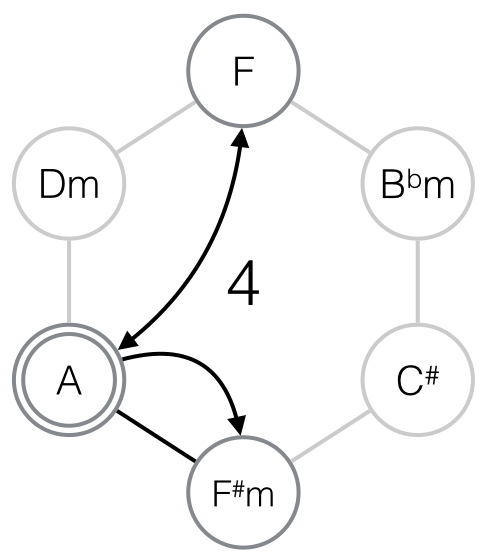
\includegraphics[width=0.5\linewidth]{STTMP_overture_1}
	\caption{ST:TMP: Overture Intro}
	\label{fg:sttmp_overture_1}
\end{figure}

\noindent\newthought{\acf{ST:TMP}} opens to a black screen accompanied by a musical overture. It portrays ''Ilia's Theme'', otherwise know as the ''Love Theme''. It is hard to find a tonic in this piece within the confines of traditional tonal music. However, I do not believe it to be of any consequence since working with film music literature often is about finding the \textit{tonal centre}. In the case of the romantic and string saturated ''Ilia's Theme'' we find the main sections moving around between four pillars; A, \ciss, F and C, each fixated in a hexatonic network. The introduction, figure \ref{fg:sttmp_overture_1} starts with what would seem to be a progression tonally unrelated to the axiom of the song, \ciss, but is in fact part of the same hexatonic \textbf{NR\(_{4}\)} circle. After \(F\sharpx{m}^{6}\Rightarrow{C\sharpx}\), a ''hollywood cadence'', the main theme starts. 
%-----------------------------------------------------------------------------
% A
%-----------------------------------------------------------------------------
\begin{figure}
\center
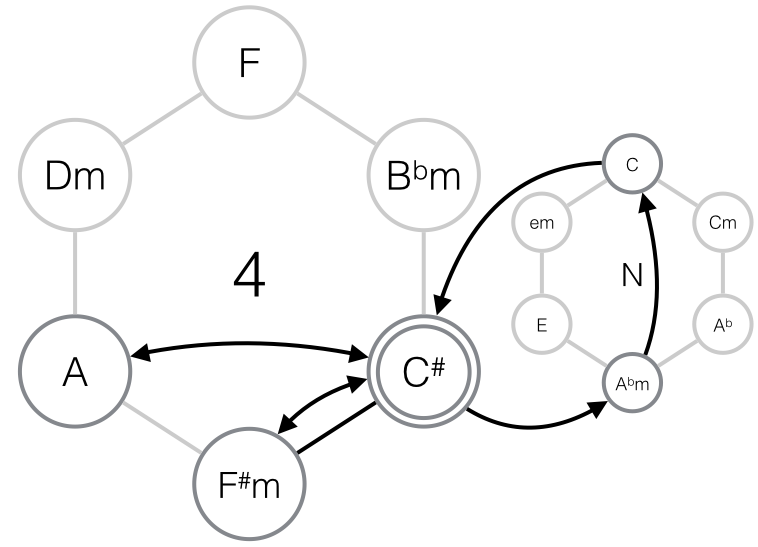
\includegraphics[width=0.7\linewidth]{STTMP_overture_2}
	\caption{ST:TMP: Overture A}
	\label{fg:sttmp_overture_2}
\end{figure}

The main theme of this cue mainly plays out in the \textbf{NR\(_{4}\)} circle. The exception is a network modulation to the \textbf{PL\(_{N}\)} circle. There is an argument to be made for view the \(G\sharpx{m}^{7(\flatx{5})}\), \textit{pc} [036t]\footnote{\keyboard{one=C,two=Diss,three=Fiss,four=Aiss,}}, as a \(E^{9}\)/\giss, but nevertheless, the main body of the chord is a \gissm \textit{transformed} with \(\flatx{5}\) (figure \ref{fg:sttmp_overture_2}).

%-----------------------------------------------------------------------------
% A'
%-----------------------------------------------------------------------------
\begin{figure}
\center
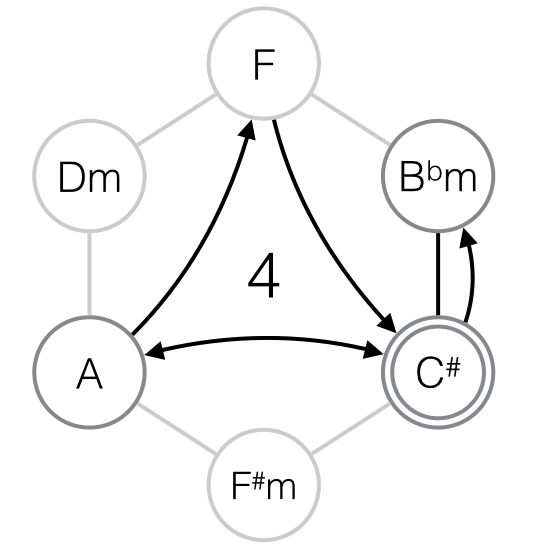
\includegraphics[width=0.5\linewidth]{STTMP_overture_3}
	\caption{ST:TMP: Overture A'}
	\label{fg:sttmp_overture_3}
\end{figure}
The second pass of A, figure \ref{fg:sttmp_overture_3}, works much in the same way, but instead of modulating outside the \textbf{NR\(_{4}\)}, Goldsmith does a minor transformation on the melody, \textbf{m.}17-18, making room for a simple \textbf{LP} to F\footnote{Which might be seen as a projection to the following part.}. The part ends with a \aissm, making it the new \(iv\), another ''hollywood cadence''. 

%-----------------------------------------------------------------------------
% B
%-----------------------------------------------------------------------------
\begin{figure}
\center
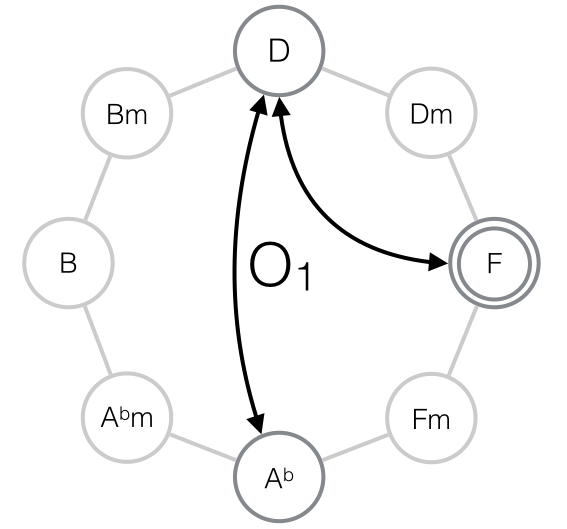
\includegraphics[width=0.5\linewidth]{STTMP_overture_4}
	\caption{ST:TMP: Overture B}
	\label{fg:sttmp_overture_4}
\end{figure}
The second part, and theme (figure \ref{fg:sttmp_overture_4}), of the cue is entirely situated in \(O_{1}\). With a pedal A acting as a coupling between F and D, acting as \(\hat{3}\) and \(\hat{5}\), Goldsmith activates a melody with a \textit{lydian} tinge before deploying a \ac{MTTP}, now famously associated with space\footnote{A term borrowed from Scott Murphy \citet{murphy_major_2006}. This progression to be treated in greater detail as I progress through this text.}.


%-----------------------------------------------------------------------------
% A''
%-----------------------------------------------------------------------------
\begin{figure}
\center
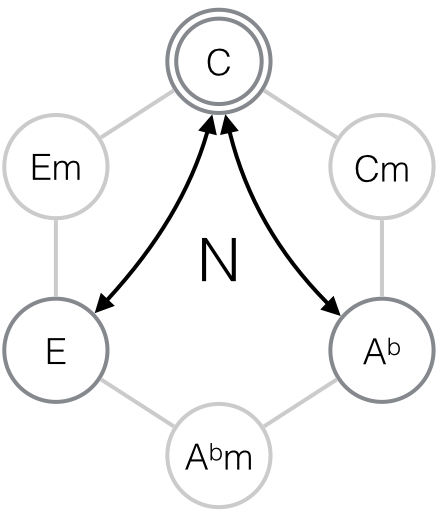
\includegraphics[width=0.5\linewidth]{STTMP_overture_5}
	\caption{ST:TMP: Overture A''}
	\label{fg:sttmp_overture_5}
	\setfloatalignment{b}
\end{figure}
When Goldsmith returns to the main theme, figure \ref{fg:sttmp_overture_5}, it is transposed to from \aflat to C, making yet another mediant modulation. The harmony is rooted in C with a pedal G. The melody uses \(\flatx{6}\), hinting at a mixolydian \(\flatx{6}\), the fifth mode in melodic minor. Through yet another mediant modulation to E Goldsmith executes the outro.


%-----------------------------------------------------------------------------
% Outro
%-----------------------------------------------------------------------------
The Outro, figure \ref{fg:sttmp_overture_6}, is a proto-projection of the now famous ''Enterprise Theme'' composed by Alexander Courage. The cadence: \(I-{\flatx}VII-IV-I\) is a \emph{subtonic plagal cadence} and is reminiscent of the old ''spaghetti'' westerns, which frequently use the \emph{subtonic half cadence}: \(I-{\flatx}VII-V-I\)\footnote{\citealt{lehman_hollywood_2013}}. It serves two purposes: (1) to project and prepare the enterprise theme and (2) to prepare the overall sonority for the main title.

\begin{figure}
\center
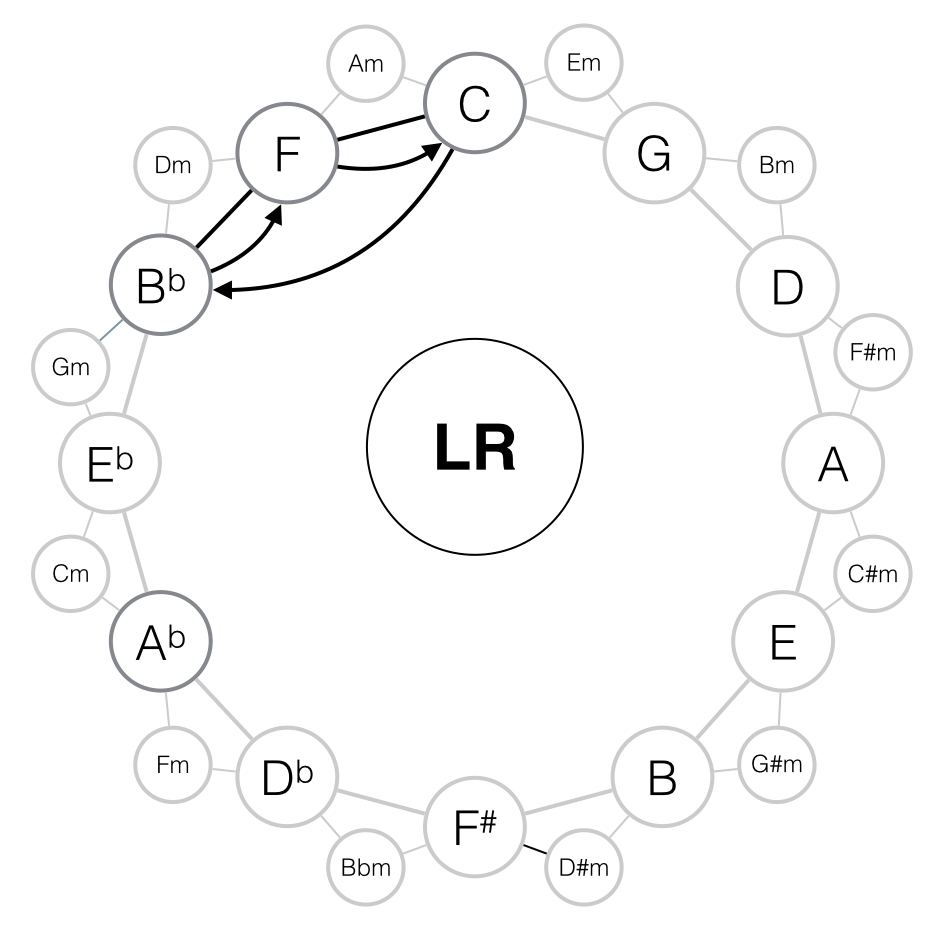
\includegraphics[width=0.7\linewidth]{STTMP_overture_6}
	\caption{ST:TMP: Overture Outro}
	\label{fg:sttmp_overture_6}
\end{figure}

%-----------------------------------------------------------------------------
% PDF
%-----------------------------------------------------------------------------
\clearpage
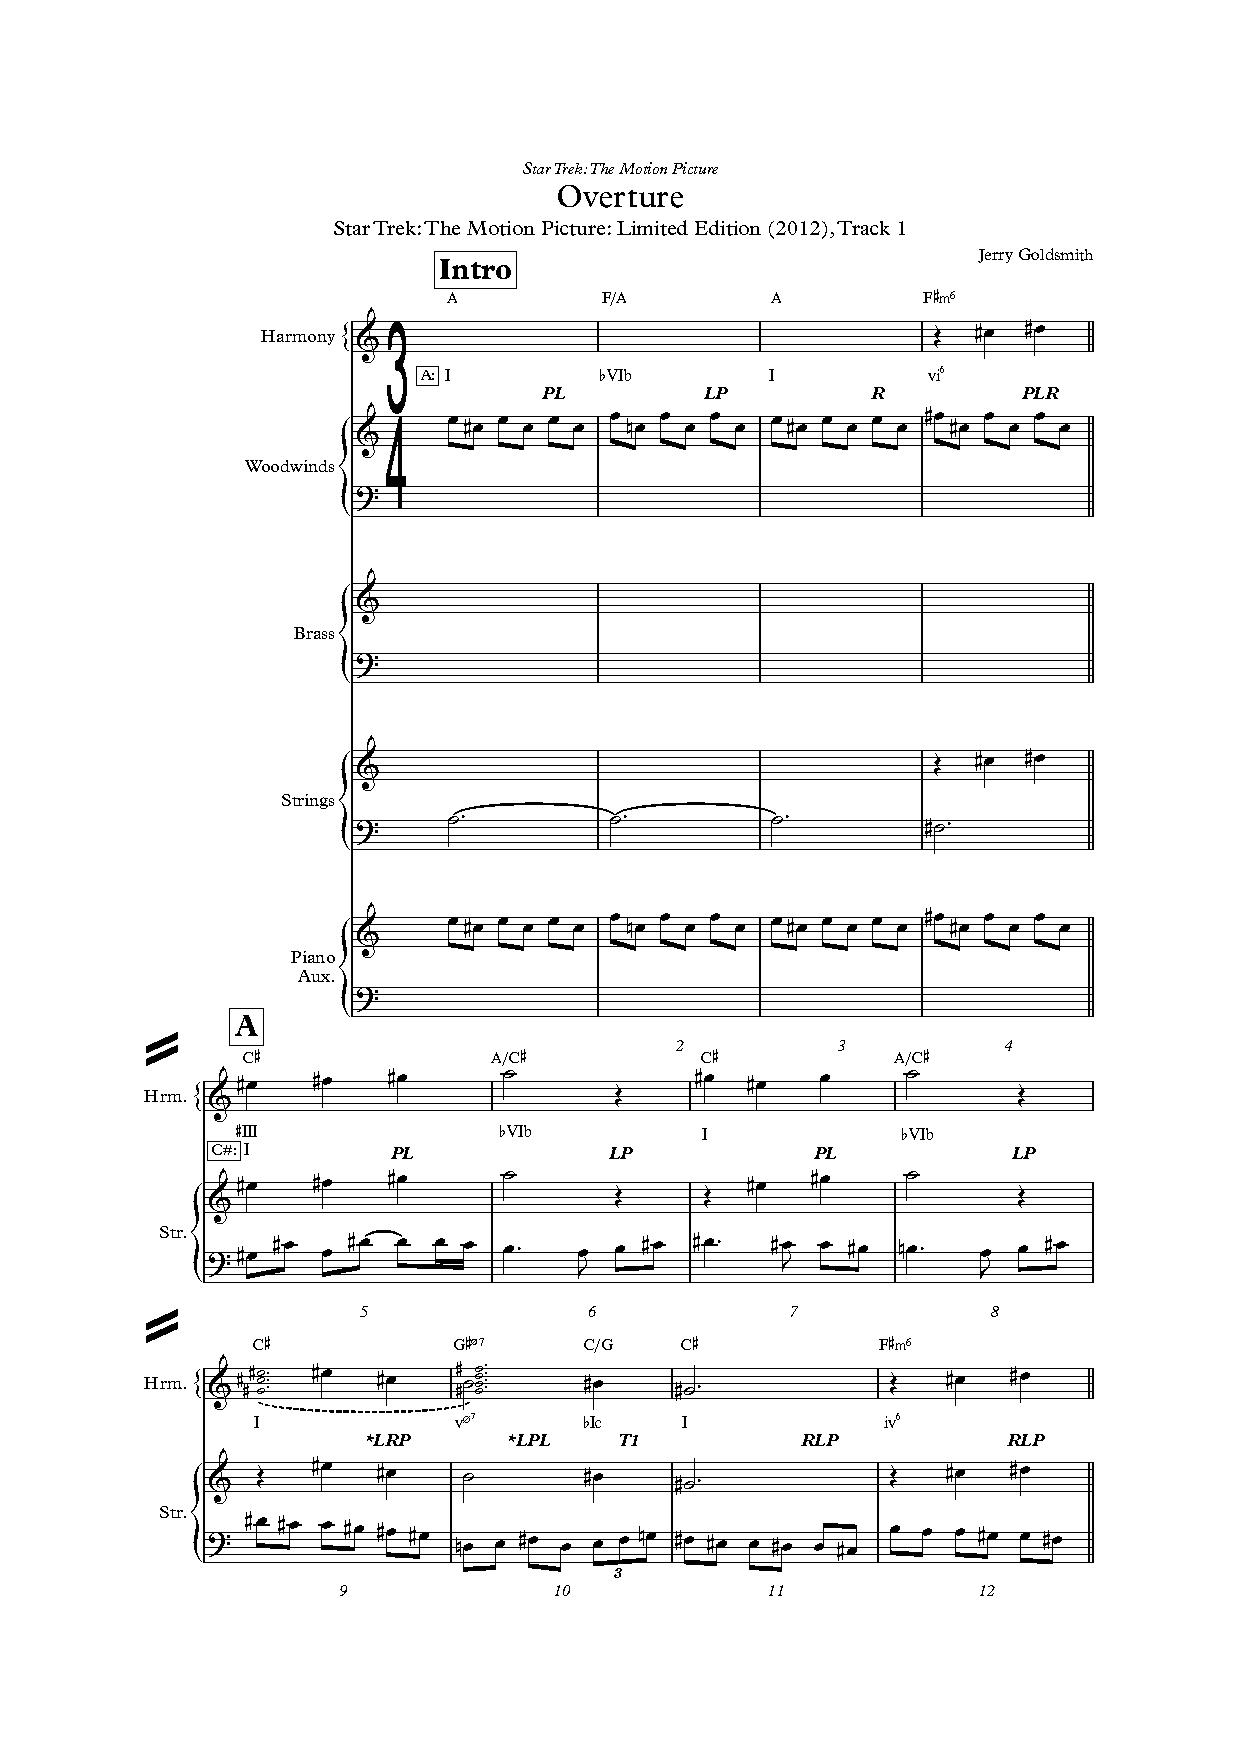
\includepdf[pages=-,pagecommand=\thispagestyle{fancy}]{pdf/st1/STTMP_Overtyre.pdf}

% Reviewed